\chapter{Secure communication channel}

\section{Encryption}

Encryption is the original goal of cryptography. It is the process of encoding messages in such a way that only authorized parties can read it. Encryption does not of itself prevent interception, but denies the message content to the interceptor.

The generic use case is: Alice and Bob\footnote{Alice, Bob and Eve are placeholder names commonly used when discussing cryptography, to identify an archetypal role of participant. Alice is a sender, Bob is a receiver and Eve is an eavesdropper. For the first time these names were used in Ron Rivest's paper introducing RSA public key cryptosystem \todo{Ref it}. Since then, a number of other names have entered cryptographic literature.} want to communicate with each other. However, communication channels are assumed not to be secure. Eve is eavesdropping on the channel. Any message that Alice sends to Bob is also received by Eve. (The same applies for messages sent from Bob to Alice, but it is the same problem and the same solution will work for Bob's messages, so we concentrate to Alice messages.) How can Alice and Bob communicate without learning everything? (\autoref{img:encryption-problem}) \cite[p.~23]{ferguson2010cryptography}

To prevent Eve from understanding the conversation, Alice and Bob are using encryption in \autoref{img:encryption}. Before they use their communication channel, they first need to agree on a cipher and a secret key.

So Alice wants to send a \textit{plaintext} message $m$. She first encrypts it using an encryption function $E(K_e, m)$ to get a \textit{ciphertext} message $c$. It can be sent over the communication channel, because only Alice and Bob know how to decrypt it. When Bob receives the ciphertext, he can decrypt it using a decryption function $D(K_e, c)$ to get the original plaintext $m$ that Alice wanted to send to him.

The cipher is preferred to be public. A well-known \textit{Kerckhoffs' principle} roughly says, that the security of the cryptosystem must depend only on the secrecy of the key, and not on the secrecy of the algorithm. They are very good reasons for this rule. Algorithms are hard to change. They are built into software or hardware, which can be difficult to upgrade. In real world, the same algorithm is used for a very long time. It is hard enough to keep the key secret, keeping the algorithm secret is far more difficult and expensive.

From past we know that it is very easy to make a small mistake and create cryptographic algorithm that is weak. If the algorithm is secret, nobody will find this fault until the attacker tries to break it. If the algorithm is kept secret, you shouldn't trust it. If the algorithm is public, researchers worldwide can participate in analyzing and improving the algorithm and its implementation.

While the cipher is publicly known, the secret key still needs to be exchanged via another communication method, which prevents Eve from reading it. Alice and Bob can meet in person to exchange the key or Alice can mail it via public post service. The key exchange problem is covered more detailed in \todo{ref it}.

\begin{figure}
  \centering
  \begin{tikzpicture}
    \node (alice) [rect,left=2.5,label={Alice}] {$m$};
    \node (bob) [rect,right=2.5,label={Bob}] {$m$};
    \node (eve) [rect,above=\nodeheight,label={Eve},label=22.5:{\noMark}] {$m$};
    \path [line,color=Gray] (alice) -| (eve);
    \path [line] (alice) -- (bob) node[pos=0.15,above]{$m$};
  \end{tikzpicture}
  \caption{How can Alice and Bob communicate securely?}
  \label{img:encryption-problem}
\end{figure}

\begin{figure}
  \centering
  \begin{tikzpicture}
    \node (alice) [rect,left=2.5,label={Alice}] {$m, c := E(K_e, m)$};
    \node (bob) [rect,right=2.5,label={Bob}] {$c, m := D(K_e, c)$};
    \path [line] (alice) -- (bob) node[pos=0.15,above]{$c$};
  \end{tikzpicture}
  \caption{Generic setting for encryption}
  \label{img:encryption}
\end{figure}



\section{Authentication}

Alice and Bob have another problem, as shown in \autoref{img:authentication-problem}. If Eve has a bit more control over the communication channel, she can not only passively listen to messages, she can also actively interfere. She can do a lot of other malicious actions. Imagine Alice sending to Bob a message containing request for bank transfer. Eve can change the message, insert a new message, delete a message so Bob never receives it, record a message and then send it to Bob later again (replay it) or reorder messages.

\autoref{img:authentication}

\begin{figure}
  \centering
  \begin{tikzpicture}
    \node (alice) [rect,left=2.5,label={Alice}] {$m$};
    \node (bob) [rect,label={Bob},label=22.5:{\noMark},right=2.5] {$m'$};
    \node (eve) [rect,label={Eve},above=\nodeheight] {$m, m'$};
    \path [line,color=Gray] (eve) |- (bob);
    \path [line] (alice) -- (bob) node[pos=0.15,above]{$m$} node[pos=0.85,above]{$m'$};
  \end{tikzpicture}
  \caption{How can Bob know who sent the message?}
  \label{img:authentication-problem}
\end{figure}

\begin{figure}
  \centering
  \begin{tikzpicture}
    \node (alice) [rect,left=2.5,label={Alice}] {$m, a := H(K_a, m)$};
    \node (bob) [rect,right=2.5,label={Bob}] {$m, a \stackrel{?}{=} H(K_a, m)$};
    \path [line] (alice) -- (bob) node[pos=0.15,above]{$m, a$};
  \end{tikzpicture}
  \caption{Generic setting for authentication}
  \label{img:authentication}
\end{figure}



\section{Public-key encryption}

\autoref{img:publickey-encryption}

\begin{figure}
  \centering
  \begin{tikzpicture}
    \node (alice) [rect,left=2.5,label={Alice}] {$m, c := E(PK_{Bob}, m)$};
    \node (bob) [rect,right=2.5,label={Bob}] {$c, m := D(SK_{Bob}, c)$};
    \path [line] (alice) -- (bob) node[pos=0.15,above]{$c$};
  \end{tikzpicture}
  \caption{Generic setting for public-key encryption}
  \label{img:publickey-encryption}
\end{figure}



\section{Digital signature}

\autoref{img:digital-signature}

\begin{figure}
  \centering
  \begin{tikzpicture}
    \node (alice) [rect,left=2.5,label={Alice}] {$m, a := S(SK_{Alice}, m)$};
    \node (bob) [rect,right=2.5,label={Bob}] {$m, V(PK_{Alice}, m, a) ?$};
    \path [line] (alice) -- (bob) node[pos=0.15,above]{$m, a$};
  \end{tikzpicture}
  \caption{Generic setting for digital signature}
  \label{img:digital-signature}
\end{figure}



\chapter{Authenticated Encryption}

\todo{popis AEAD}

\section{Block cipher modes}

from 70s

\begin{description}
  \item[ECB]
  \item[CBC]
  \item[CFB]
  \item[OFB]
  \item[CTR]
\end{description}

\todo{Block cipher modes image from @angealbertini}

Exploiting malleability:

ECB: Rearrange, replay blocks
CTR, OFB: Bitwise modification of blocks
CBC: Change current ciphertext block to predictably change the next plaintext block (during decryption)

Chosen-boundary attacks:

ECB, CBC, CFB: Partial chosen-plaintext control
Decrypt messages byte by byte

Here come the XOR ninjas

\section{Authenticated Encryption}
\section{Authenticated Encryption with Associated Data}



\section{Generic compositions}

\begin{description}
  \item[Encrypt-and-MAC]
  \item[MAC-then-Encrypt]
  \item[Encrypt-then-MAC]
\end{description}

\begin{figure}
  \centering
  \begin{subfigure}[b]{0.3\textwidth}
    \centering
    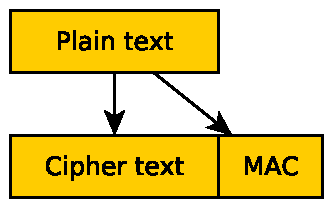
\includegraphics[width=0.9\textwidth]{images/encrypt-and-mac.pdf}
    \caption{Encrypt-and-MAC}
  \end{subfigure}
  \begin{subfigure}[b]{0.3\textwidth}
    \centering
    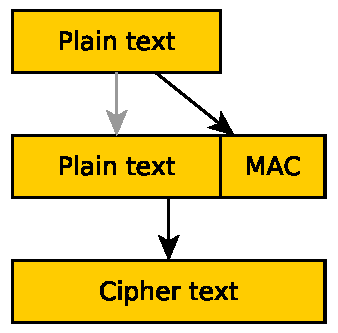
\includegraphics[width=0.9\textwidth]{images/mac-then-encrypt.pdf}
    \caption{MAC-then-encrypt}
  \end{subfigure}
  \begin{subfigure}[b]{0.3\textwidth}
    \centering
    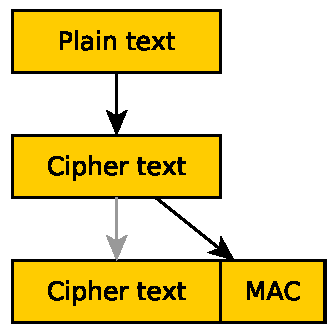
\includegraphics[width=0.9\textwidth]{images/encrypt-then-mac.pdf}
    \caption{Encrypt-then-MAC}
  \end{subfigure}
  \caption{Generic compositions of Authentized Encryption}
\end{figure}

\section{Competition for Authenticated Encryption: Security, Applicability and Robustness}

CAESAR is worldwide cryptographic competition, focused on finding new methods of authenticated encryption, that offer advantages against commonly used AES-GCM and will be suitable for widespread adoption. Submitted algorithms will be publicly evaluated by committee of researchers in fields of cryptography and cryptoanalysis.

\todo{popis algoritmů byly v soutěži, v čem se lišily, jaké a jak v nich byly nalezeny zranitelnosti a proto nepostoupily}

\todo{výběr algoritmu pro implementaci}

\subsection{Selection criteria}

\begin{description}
  \item[Online (one-pass)]
\end{description}



\subsection{NORX}

NO(T A)RX

ARX - Addition, Rotation, XOR

\subsubsection{Design goals}

\begin{itemize}
  \item \textbf{High security}
  \item \textbf{High speed} (in SW \textit{and} HW)
  \item \textbf{Simplicity} (of spec \textit{and} code)
  \item Online / one-pass
  \item Scalability (parallelism, unrolling)
  \item High key agility (no "key schedule")
  \item Side-channel leaks robustness (esp. timings)
\end{itemize}

\subsubsection{Parameters}

\begin{description}
  \item[Word Bit Size] $W \in {32, 64}$
  \item[Number of Rounds] $1 \leq R \leq 63$
  \item[Parallelism Degree] $0 \leq D \leq 255$ (0?)
  \item[Tag Bit Size] $|A| \leq 10W$
\end{description}

\begin{table}
  \centering
  \csvreader[
    after head=\begin{tabular}{llll}\toprule\csvlinetotablerow\\\midrule,
    late after line=\\,
    late after last line=\\\bottomrule\end{tabular}
  ]
    {tables/norx-proposed-instances.csv}{}
    {\texttt{\csvcoli} & \csvcolii & \csvcoliii & \csvcoliv}

  \caption{NORX proposed instances}
\end{table}

R=6: higher security margin

D=4: high throughput on parallel architectures

\input{text/aead-caesar-selection.tex}


